\section{Realios mašinos projektas}

\subsection{Techninės įrangos komponentai}

\begin{description}
  \item[Procesorius]\leavevmode \\
Procesorius gali dirbti dviem rėžimais: vartotojo ir supervizoriaus. Registras MODE nusako procesoriaus rėžimą(0 - vartotojo, 1 - supervizoriaus)
\begin{itemize}
  \item Vartotojo rėžimas - jame yra vykdoma paduota programa
  \item Supervizoriaus rėžimeas - jame komandos iš supervizorinės atminties yra betarpiškai apdorojamos aukšto lygio kalbos procesoriaus
\end{itemize}
Procesoriaus registrai:
\begin{itemize}
  \item R1 - 4b bendro naudojimo
  \item R2 - 4b bendro naudojimo
  \item IC - 2b komandų skaitliukas
  \item PTR - 4b puslapių lentelės registras skirtas puslapiavimui
  \item CH1, CH2, CH3 - 1b atitinkamų kanalų registrai. 0 - kanalas laisvas, 1 - kanalas užimtas
  \item PI - 1b programinių pertraukimų registras\leavevmode
		\\1 - pažeista atminties apsauga
		\\2 - neatpažintas operacijos kodas
           	\\3 - taimerio registras pasiekė 0
		\\4 - dalyba iš 0
		\\5 - Aritmetinės operacijos klaida
  \item SI - 1b supervizorinių pertraukimų registras\leavevmode
		\\1 - GD(GetData) komandos pertraukimas
		\\2 - PD(PrintData) komandos pertraukimas
		\\3 - HALT komandos pertraukimas
  \item TI - 1b taimerio pertraukimo registras
  \item IOI - 1b įvedimo/išvedimo operacijos pabaigos pertraukimas. 1 - pirmas kanalas, 2 - antras kanalas, 4 - trečias kanalas
  \item MODE - 1b rėžimo registras. 0 - dirbama vartotojo rėžimu, 1 - dirbama supervizoriaus rėžimu
\end{itemize}

  \item[Naudotojo atmintis] \leavevmode \\
Atmintis, skirta virtualių mašinų atmintims bei puslapių lentelėms saugoti. Ji turi 256 žodžius, nuo 00 iki FF. Žodžio ilgis - 4b
  \item[Supervizorinė atmintis] \leavevmode \\
Atmintis, skirta operacinės sistemos poreikiams, laikanti sisteminius procesus, kintamuosius, resursus ir t.t Realizuojama aukšto lygio programavimo kalba

\item[Puslapiavimo mechanizmas] \leavevmode \\
Sąryšis tarp virtualios atminties ir realios amtinties bus palaikomas per puslapiavimo mechanizmą. Virtualios mašinos puslapį(bloką) sudaro 16 žodžių.
\\ Registre PTR bus saugomas einamosios puslapių lentelės ilgis bei adresas. Keturi PTR baitai a0, a1, a2, a3 bus paskirstyti taip:
\begin{itemize}
\item a0 - nenaudojamas(tuščias)
\item a1 - puslapių lentelės ilgis - 1
\item a2 - naudojamas kartu su a3 gauti puslapių lentelės adresą pagal: a2*10 + a3
\item Dviženklis adresas [x1, x2]  virtualioje adresinėje erdvėje aparatūriškai advaizuojamas į realų adresą vartotojo atmintyje: 10*[10*(10*a2 + a3) +x1] + x2
\end{itemize}

  \item[Duomenų perdavimo kanalai] \leavevmode \\
Kanalai yra specialūs procesoriai, valdantys įėjimo, išėjimo ir išorinės atminties įrenginius, dirbantys lygiagrečiai su centriniu procesoriumi.
\begin{itemize}
  \item CH1 - paima duomenis iš įvesties įrenginio(šiuo atveju - flash atmintinės) ir perduoda iš buferio į realią atmintį
  \item CH2 - apdoroja duomenų srautą einantį iš realios atminties į išvedimo įrenginį(šiuo atveju - spausdintuvą)
  \item CH3 - apdoroja apsikeitimą duomenimis tarp supervizorinės atminties ir kietojo disko tiek skaitymo, tiek rašymo kryptimis
\end{itemize}
Visi kanalai centriniame procesoriuje turi atitinkamus 1b registrus CH1, CH2, CH3. 0 - kanalas laisvas, 1 - kanalas užimtas.


  \item[Įvedimo ir išvedimo įrenginiai] \leavevmode \\
Įvedimo įrenginys - flash atmintinė, išvedimo įrenginys - spausdintuvas. Abu turi 16 žodžių dydžio buferius apsikeisti duomenimis. Užpildžius buferį, jis yra siunčiamas
į išvedimo įrenginį arba į kanalą priklausomai nuo situacijos.



\end{description}

\subsection{Realios mašinos techninės įrangos komponentų išsidėstymo vienas kito atžvilgiu ir tarpusavio sąveikos schema}
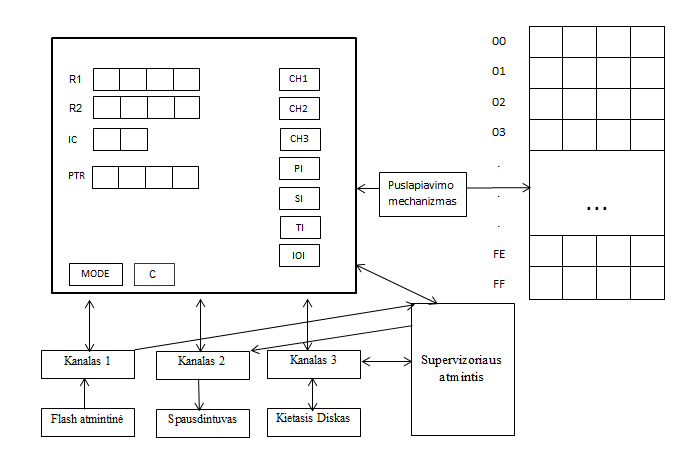
\includegraphics{RM.PNG}
